\documentclass[.../main.tex]{subfiles}

\begin{document}

	This chapter describes a proposed line of research which aims
        to study the evolution of swarm systems with independent,
        learning agents under the influence of predictive controls. We
        detail the novel lines of research which this work aims to
        undertake, providing suggestions of the hypotheses posed by
        these lines. With this in mind the following studies are
        proposed and developed subsequently:

	\begin{itemize}
		\item \textbf{Stability and Chaos in MARL:} in which
                  we seek to understand the dynamics of agent
                  strategies when using Q-Learning to learn a game
                  through iteration. We will establish the stability,
                  as a function of parameters, when learning general
                  p-player N-action games.  This study enables the
                  appropriate selection of parameters and payoff
                  matrices to ensure the stability of the strategies
                  of a finite set of agents, such as leaders in a
                  swarm.

                  \fr{this is already attempted in the currect
                    research section, isn't it?}

              \item \textbf{Dynamics of Mean-Field Q-Learning Games:} in which we examine the
		strategy dynamics for large populations of agents learning through iterated games and
		mean-field Q-Learning. We seek to understand the long term behaviour of such mean-field
		systems in terms of its strategy selection. This study extends the previous and allows for
		the stability of the strategies of a population of agents to be established.
		\item \textbf{Model Predictive Control of Active Particles through Fields:} in which we
		investigate the interaction of a swarm of active particles with potential fields. We
		establish the stabilisability of an MPC scheme with defined stage costs, as well as an
		analysis of the suboptimality of the method.
		\item \textbf{Incorporation of Intelligence in Control:} in which we adapt the dynamical
		system from the above point to include an interaction term, accounting for strategy
		selection by agents who learn through iterated games against one another. Interactions with
		an MPC scheme is then to be examined in a similar capacity.

	\end{itemize}

        \fr{we analyze each topic in a section \ldots}

	% \textbf{TODO: Ensure all references here are in the Lit Review}

    \section{Stability and Chaos in MARL} \label{sec::Chaos_in_MARL}

    This segment of research is aimed towards a deeper understanding
    of the strategy evolution of agents following a Q-Learning
    approach. This allows for guarantees to be placed on the behaviour
    of such agents, in particular the conditions under which the game
    will converge to a stable equilibrium.

    It has long been established that, upon lifting the strong
    assumptions made by traditional game theory (such as the
    rationality of agents and complete information), that player
    strategies can result in much more complex behaviour than
    convergence to a Nash Equilibrium (NE). In fact, this is even true
    on what would commonly be regarded as 'simple' games such as
    tic-tac-toe and prisoner's dilemma \cite{Galla2011,
      Sato2002}. These behaviours include: convergence to a unique
    equilibrium (though not always to an NE), convergence to one of
    multiple equilibria, limit cycles and chaos. These behaviours are
    shown in Figure \ref{fig::DynamicalBehaviours} Of these, the most
    preferable is, of course, convergence to a unique equilibrium,
    although it is still possible to study systems with multiple
    equilibria or limit cycles \cite{Strogatz2000}. However, it would
    be difficult to control systems whose dynamics are governed by
    chaos (though research into controlling chaos is ongoing and rife
    with opportunity \cite{Fradkov2009}) and so MARL techniques should
    avoid this. It would, therefore, be a useful endeavour to
    determine the conditions under which these sorts of behaviours
    arise.

    \begin{figure}[h]
    	\centering
    	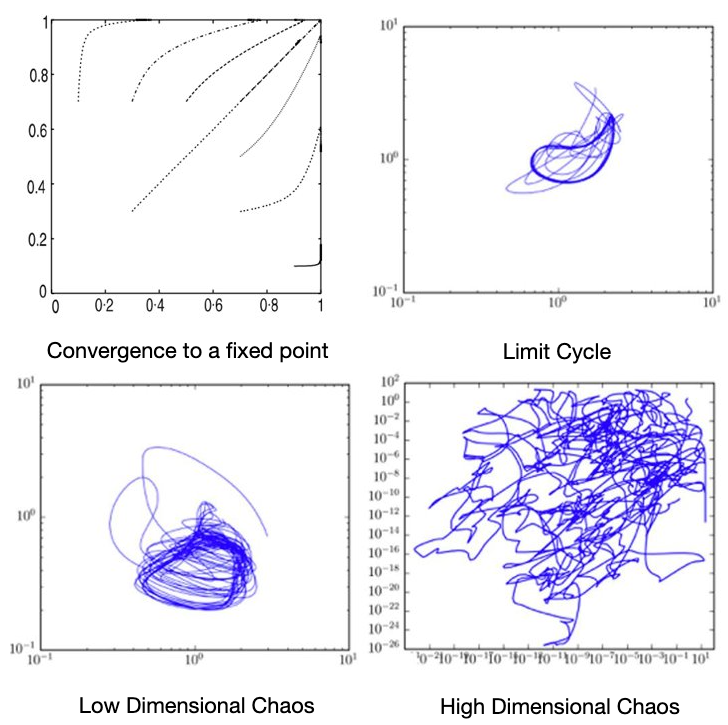
\includegraphics[width=1.1\textwidth]{Figures/DynamicalBehaviours}
    	\caption{ \label{fig::DynamicalBehaviours} Different types of
          dynamial behaviour displayed by learning agents. a)
          Convergence to a unique fixed point in the upper right
          corner (1, 1). This fixed point is unique, in that all
          trajectories, regardless of initialisation, will converge to
          this point \cite{Tuyls2006AnGames}. b) Limit Cycle, the
          trajectories converge to cyclic behaviour c, d) Chaotic
          behaviour, here small deviatons in the initial conditions
          can grow exponentially \cite{Sanders2018}.}
    \end{figure}

    The behaviour of a system may be studied given a model of its
    dynamics. It is through this process that a wide array of physical
    systems, from harmonic pendulums to geophysical fluids, can be
    understood. A growing body of research aims to understand
    multi-agent reinforcement learning through the lens of its
    dynamics. In this light, Tuyls et al. \cite{Tuyls2006AnGames} were
    able to derive a model of the strategy evolution of agents
    learning through iterated games.  Through this, they were able to
    arrive at the following model of Multi-Agent Q-Learning

	\begin{subequations}
	\label{eqn::EOM}
		\begin{equation}
			\frac{\dot{x}(t)}{x(t)} = \alpha \tau (\sum_{j} a_{ij} y_j - \sum_{i j} x_i a_{ij} y_j)
			+ \alpha \sum_j x_j ln(\frac{x_j}{x_i}) 
		\end{equation}
		\begin{equation}
			\frac{\dot{y}(t)}{y(t)} = \alpha \tau (\sum_{j} b_{ij} x_j - \sum_{i j} y_i b_{ij} x_j)
			+ \alpha \sum_j y_j ln(\frac{y_j}{y_i}).
		\end{equation}
	\end{subequations}

        \fr{I understand the equations are the same as in the previous section. I suggest we move the explanation there and remove it from here.}

	Here, $\alpha$ and $\tau$ are the parameters of the agent;
        Sanders et al. refer to these as the memory and intensity of
        choice parameters respectively. Agent 1 takes action i with
        probability $x_i$ while Agent 2 takes action j with
        probability $y_j$. If these actions are taken, the agents
        receive payoff $a_{ij}$ and $b_{ji}$ respectively. With these
        equations, it is possible to predict the expected behaviour of
        Q-Learning agents, as shown in Figure
        \ref{fig::TuylsExperiments}.

	\begin{figure}[h]
		\centering
		\begin{subfigure}[b]{0.9 \textwidth}
			\centering
			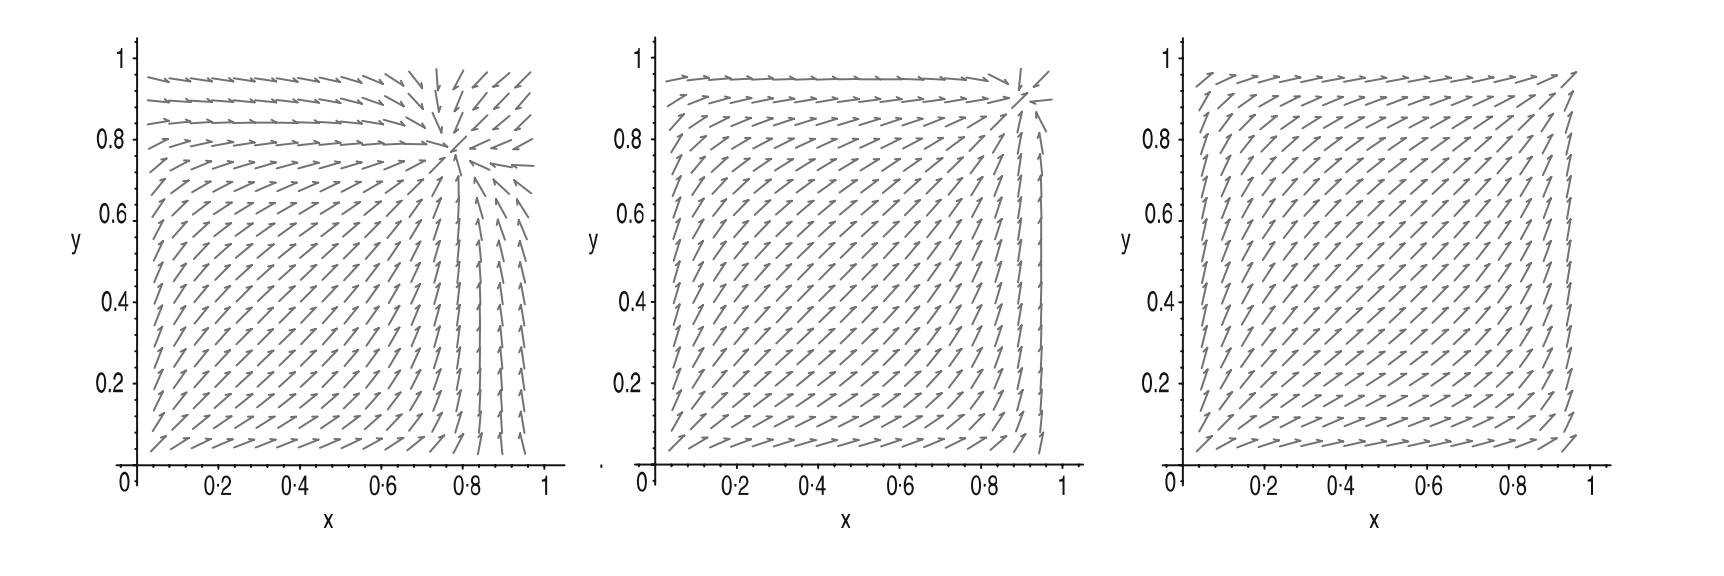
\includegraphics[width=0.75 \textwidth]{Figures/Dynamics}
			\caption{}
		\end{subfigure}
		
		\begin{subfigure}[b]{0.9 \textwidth}
			\centering
			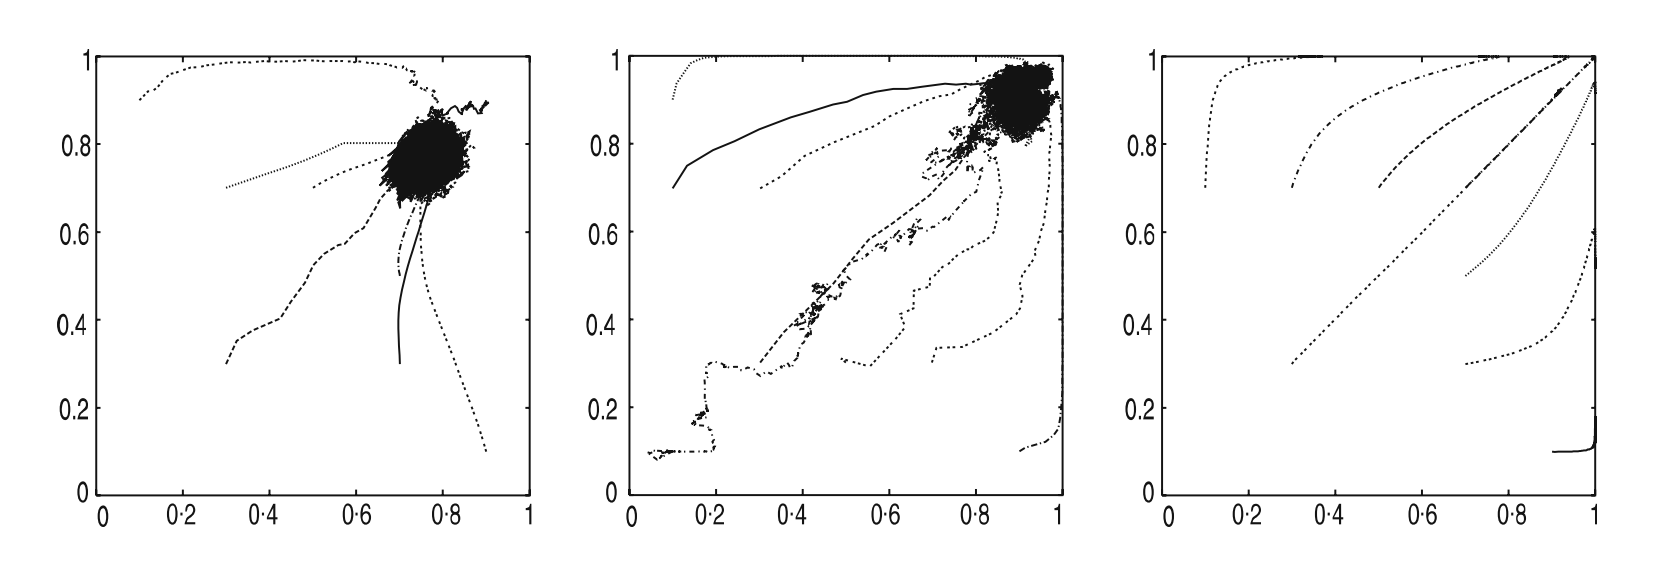
\includegraphics[width=0.7 \textwidth]{Figures/Q-Learners}
			\caption{}
		\end{subfigure}

		\caption{ \label{fig::TuylsExperiments} Figures taken from \cite{Tuyls2006AnGames} a) Phase
		plot showing the expected behaviour of Q-Learning agents trained by iterating the
		Prisoner's Dilemma game as predicted by (\ref{eqn::EOM}). From left to right, the agents
		have parameter $\tau = 1, 2, 10$. b) Corresponding trajectories of Q-Learning agents with
		randomised initial conditions displayed through numerical simulation. It is clear that the
		trajectories in b) follow the predictions in a), after stochasticity is accounted for. }
	\end{figure}	

	It is clear, both from (\ref{eqn::EOM}) and Figure \ref{fig::TuylsExperiments} that the long-term strategy selection of
	these agents is determined by the parameters $\alpha, \tau$ and the payoffs $a_{ij}, b_{ij}$. We
	then pose the question: how do these elements influence the types of behaviours seen during
	learning on an iterated game? In other words, under what parameter selections are we likely to
	see convergence to unique equilibria, multiple equilibria, limit cycles or chaos?

	With this in mind, the intention of this area of study is to consider the analysis presented in
	works such as \cite{Sanders2018} and \cite{Galla2011}. Here, the authors examine the
	Experience Weighted Attraction (EWA) algorithm, which is regarded as a strong model for the
	learning behaviour of human players in a game \cite{Camerer2009}. The authors are able to
	determine the regions of parameter space in which complex behaviour,
	including cycles and chaos, predominantly occur and those in which a given game converges to a
	stable equilibrium. Figure \ref{fig::GallaPredictions} reproduces the graphs shown in \cite{Sanders2018} which
	illustrates the successful derivation of a 'phase line', across which learning shifts from
	convergent to chaotic.

    \begin{figure}[h]
    	\centering
    	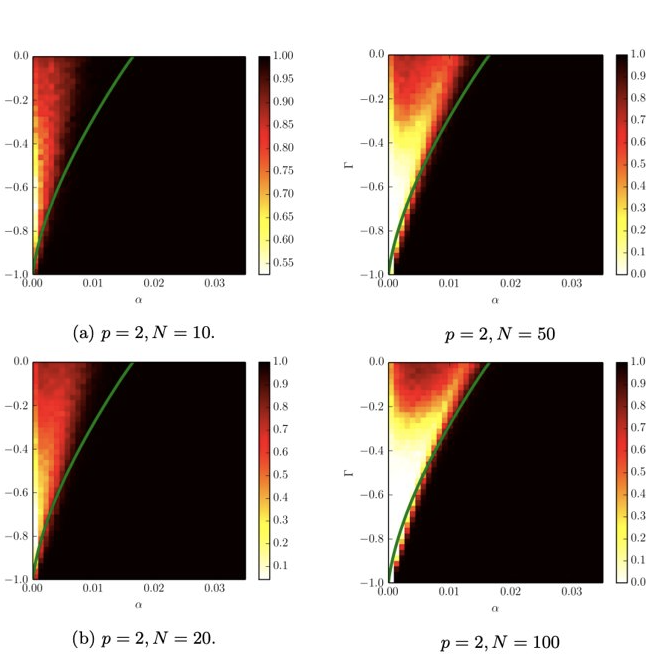
\includegraphics[width=0.6\textwidth]{Figures/GallaPredictions}
    	\caption{ \label{fig::GallaPredictions} Results as produced in the supplementary material
    	of Sanders et al \cite{Sanders2018}. Here, $p$ is the number of players, $N$ is the number
    	of actions, $\Gamma$ represents the competitiveness of the game (-1 represents zero-sum, 1
    	represents shared rewards) and $\alpha$ is the memory parameter of the agent as before.
    	Here $\tau$ is held constant at 0.05 (though it is referred to as $\beta$ in the paper).
    	The black region represents where games converged to a fixed point through all simulations,
    	whilst the hotter regions represent the more complex dynamics - red shows the presence of
    	limit cycles and white regions signal the onset of chaos. The green line is a theoretical
    	estimation for the phase line which separates the convergent dynamics from complex.}
    \end{figure}

    We propose to bridge the analysis presented by Sanders
    et al. and Galla et al. towards games learnt using MARL, particularly Q-Learning with
    Boltzmann exploration as considered by Tuyls et al. This would allow for a characterisation of
    the expected resultant behaviour under given parameters for a particular game. The vision for
    this is to provide guarantees on the stability of a finite set of agents within a swarm, such as
    leaders in a flock. Without this, it would be impossible to ensure the stability of a swarm in
    which intelligent, social interactions must be accounted for. However, this analysis
    would also allow for a characterisation of the conditions under which MARL algorithms may
    feasibly be applied, thereby supporting the ability of researchers and engineers to choose their
    payoff matrices and parameters accordingly.

    This segment of research is currently underway and approaching completion. The analysis was
    described in Section \ref{sec::Chaos_in_Q-Learning}.

    \fr{I would move all of the above to the previous section.}

    \section{Large Population Dynamics} \label{sec::Large_Agent_Dynamics}

    This segment of research aims to model the game dynamics of large
    populations of agents learning through iterated games and
    mean-field Q-Learning. The aim is to provide similar guarantees of
    stability as in the previous sections with the caveat that all
    agents in the population can learn, rather than a finite subset.

    One of the main results shown by Sanders et al. \cite{Sanders2018}
    is that as the number of players in a game increases, the learning
    behaviour is more likely to be chaotic, regardless of the choice
    of parameters. This is intuitive since a higher number of players
    would result in a greater strategy space and more agents for any
    particular player to learn against and is verified by their
    presented results as in Figure \ref{fig::GallaPrevalence} - the
    hotter regions occupy a larger area as \fr{?}

    \begin{figure}[h]
    	\centering
    	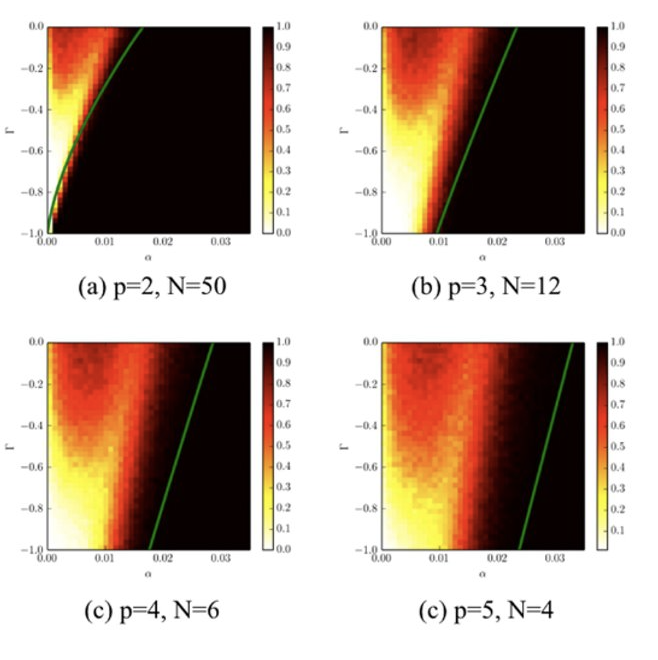
\includegraphics[width=0.6\textwidth]{Figures/GallaPrevalence}
    	\caption{ \label{fig::GallaPrevalence} Results as produced in
          the supplementary material of Sanders et al
          \cite{Sanders2018}. The same items appear here as in Figure
          \ref{fig::GallaPredictions}, except the value of p (number
          of players) increases moving from top left to bottom
          right. It is clear that the hotter region occupies a larger
          region of parameter space, indicating that as the bumber of
          players in the game increase, chaos becomes more prevalent.}
    \end{figure}

    Yet it can be argued that, for large populations of agents (e.g.,
    a crowd), the aggregate behaviour may be predictable \fr{provide some justification to this claim?}. This
    intuition is the foundation upon which crowd dynamics and flocking
    systems are based. In fact, the work presented by Leung et
    al.~\cite{Hu2019} provides a cursory verification of this
    intuition. Here, the authors present an analysis of the learning
    dynamics for a large agent population (which they approximate as
    containing infinite agents) where each agent is an independent
    Q-Learning using Boltzmann action selection. The result is a
    system of equations, governed by a Fokker-Planck model which is
    numerical shown to be a strong predictor of the overall strategy
    selection of the population. Indeed, rather than examining the
    strategies of every agent in the population (which the authors
    approximate as infinitely large), they model the evolution of a
    probability density function which, for each action, defines the
    density of agents who retain a given Q-value for that action. This
    is illustrated in Figure \ref{fig::LeungPredictions}.

    \begin{figure}[h]
    	\centering
    	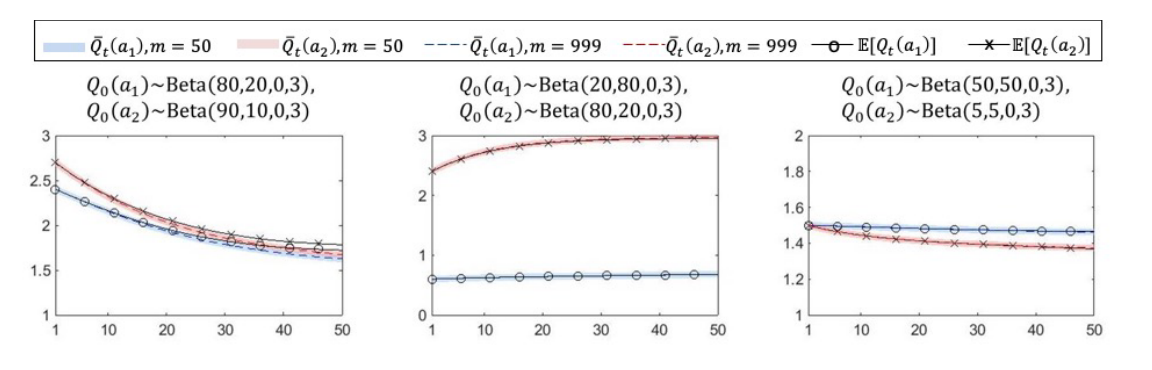
\includegraphics[width=0.9\textwidth]{Figures/LeungPredictions}
    	\caption{ \label{fig::LeungPredictions} Results as produced in Leung et al \cite{Hu2019}.
    	Here, the solid and dotted lines represent the evolution of thhe expectation of Q-values of
    	two actions across a population of 50 or 999 agents respectively who are trained on an
    	iterated Stag Hunt game. The circled and crossed
    	lines represent the dynamics of these Q-values as predicted by the system of equations
    	derived in the paper. These are seen to closely match the results of the numerical
    	experiments.}
    \end{figure}

   	As the authors point out, this is the first attempt at considering such a problem, and relies on
	heavy assumptions. The strongest of these is placed on the game itself, which is always
	assumed to be cooperative (in Sanders' terms, $\Gamma = 1$). We, therefore, propose extending
	this model to accomodate an arbitrary choice of games. 

	The following are suggestions for approaching the estimation of large population dynamics.

	\begin{itemize}
		\item Estimate the population state through Random Finite Sets (RFS) and
	apply the models from the previous study. The aim here is to determine a state
	estimation for a swarm of unknown size through a random finite set by solving
	an optimal estimation problem  (typically iterated through a Kalman Filter
	\cite{Doerr2019}. As the swarm is treated probailistically, the theory can
	accomodate an arbitrarily large system. Importantly, this may allow for the
	results from the previous section to be leveraged towards an arbitrary
	population. 

	\item Decompose a generic game into a weighted sum of a
	competitive and a cooperative game. Treat these as two separate agents and
	invoke the mean field approximation (MFA) so that any given agent is
	effectively engaged in a three-player game where the strategy of the opponents
	is the average strategy of the population. This leverages the existing results
	on the dynamics of three body problems in game theory \cite{Nagarajan2018} in
	a mixture of co-operative and competitive settings.
	\end{itemize}

	
	%\textbf{TODO: Elaborate on the technical details of the RFS and three body hypotheses}


    \section{Swarm Control through Fields} \label{sec::Swarm_Field_Control}

    Here we aim to study the interaction of a swarm of 'active particles' with a potential field. In
    particular this field is to be generated by 'field particles'. A model predictive control 
    (MPC) scheme
    is to be devised to drive this system to desired configurations, with guarantees placed on
    stability and satisfaction of input constraints. The sub-optimality of the control
    scheme is to be studied.

    As described in the previous chapter, the control of swarms has been examined through the use of
    mean field models. These models resolve the fact that it is impossible to view the entire system
    as simply the sum of all of the agents and rather model the overall state of the system through
    density functions. Controls are then applied to this function whose evolution is described
    through, typically, one of two partial differential equations: the Fokker-Planck Equation (also
    referred to as the Kolmogorov Forward Equation) and the Vlasov Equation. The former has seen
    some success in recent literature \cite{Elamvazhuthi2019, Li2017,
    Roy2017}, though it makes the assumption that the system evolves through 'drifted
    brownian motion'. This means that the agents are considered to move about independently and
    randomly, though under the influence of a field which affects their velocity. This technique
	has been shown, both theoretically and experimentally, to drive swarm systems in a stable
	manner \cite{Fleig}. The latter is beginning to show promise 
	though control is typically through leadership rather than fields \cite{Burger2019}. 

	The hypothesis of this section is that the distribution of active particles, whose evolution is
	described through a Vlasov equation, may be controlled through the influence of a scalar field
	generated by 'field paricles'. This is drawn from the dynamics posed by Bellomo et al. 
	\cite{Bellomo2017}

	\begin{equation}
	\label{eqn::Vlasov}
    \begin{split}    
        \partial_t f + \Vec{v} \cdot \nabla_{\Vec{x}} f + \kappa \nabla_{\Vec{v}} \cdot (F_a (f) f)
        = \epsilon Q(f, f) \quad  (\Vec{x}, \Vec{v}) \in \Omega[f] \times D_{\Vec{v}}, \quad t>0, \\
        F_a[f](t, \Vec{x}, \Vec{v}) = - \int_{\Omega [f] \times D_{\Vec{v}}} \psi (|\Vec{x} - \Vec
        {x^*}|)(\Vec{v} - \Vec{x^*}) f(t, \Vec{x}^*, \Vec{v}^*) d\Vec{x}^* d\Vec{v}^*, 
    \end{split}
    \end{equation}


    Here, $f = f(t, \Vec{x}, \Vec{v})$ is the one-particle probability density function at
    phase-space position ($\Vec{x}, \Vec{v}$), $\Vec{v}$ and time $t$ which represents the state of
    the system. $\kappa \geq 0$ is a scalar
    coefficient, $\psi$ denotes the communication strength between particles, and ($\Vec{x}^*, \Vec
    {v}^*$) gives the position in phase space of a 'field particle'. It can be seen that the these
    field particles influence the velocity of the swarm agents.

	The contribution that this study presents over those using brownian motion is the inclusion of an
	interaction operator $Q(f, f)$. This governs how agents interact with one another. With this
	term included, the dynamics account for the tendency of agents to avoid collisions. However,
	the term is intended to account also for social interactions between agents, which we aim to
	leverage in the subsequent section.

	The complexity of this interaction term will need to be gradually increased over time. To begin
	with, we may entirely neglect this term. It is here that we will compare the model proposed by Zhang
	with that proposed by Bellomo et al. We may then consider only local interactions, which is typical
	for most swarming systems in the current literature, before then considering non-local interactions.
	This provides the scope for swarms to interact with a greater number of agents. At this stage, we
	may expand our study to consider the presence of interaction domains. This places constraints on how
	agents may interact with one another, allowing for a greater generalisation of inter-agent
	interactions. Ultimately, we would like to influence the interaction term, though this is discussed
	in Section \ref{sec::Intelligence_in_control}. The questions we will
	consider here are:

	\begin{itemize}
		\item The stablity of the system: Under what conditions is it possible to drive the
		swarm from one configuration to another in a stable manner? Fortunately, Bellomo et al
		present a candidate lyapunov functional upon which dissipation can be evaluated, though it
		will need to be adapted for the consideration of the consensus models.
		\item The guarantees of the system: Is it possible to ensure that controls remain within an
		admissible set (typically a closed, bounded and convex set \cite{Fredi2010}).
		\item Whether the conservation laws of normalisation and total mass, as presented in 
		\cite{Bellomo2017} can be guaranteed.
	\end{itemize}

	These results will be established theoretically alongside the sub-optimality of the MPC scheme
	and verified through numerical simulations in a 2D environment. It
    will be of interest to perform a similar analysis to Ko and Zuazua \cite{Ko2019} in which the
    cost functional is altered to favour particular metrics  (e.g. running cost, control time etc.)
    and also analyse the effect of varying the time horizon.

    \section{Incorporation of Intelligence in Control} \label{sec::Intelligence_in_control}

    This section of the study is perhaps the strongest extension
    proposed in this chapter, and will likely be the most
    challenging. Here, we examine the dynamics (\ref{eqn::Vlasov}) in
    which the interaction term accounts for the social dynamics of the
    decision making of individual agents who have learnt through an
    iterated game. We leverage the strategy evolution dynamics and
    stability analysis established in \ref{sec::Chaos_in_MARL} and
    \ref{sec::Large_Agent_Dynamics}.

	Two proposals for incorporation of social interaction:
	\begin{itemize}
		\item Addition of the agent decisions as a constant in the state $f$. This will require that
		the decisions remain fixed in the state and so it will be required to make sure that the
		controls have no influence on this element.
		\item Weighted summation term in the probability of an agent changing its velocity from
		$v_*$ to
		$v$ due to a field particle with velocity $v^*$ $A[f](v_* \rightarrow v | v_*, v^*)$.
		Here, weights are equal to the agent strategy. This extends to both the swarms in
		which the leaders are making decisions (only leaders have this term) as well as in
		swarms where the population makes decisions (everyone has this term). This will need to be
		done with care though to ensure that normalisation holds. Note that, as this a probabilistic
		approach, we will need to examine the stochastic behaviour of the system and the extent to
		which constraint and conservation satisfaction can be guaranteed.
	\end{itemize}

	The MPC scheme from the previous section will then be adapted to this dynamical system with the
	same questions of well-posedness and stability considered. 

	A possible extension of this would be to consider online learning by incorporating the time
	evolution of the strategy space within the social interaction term, which would now be
	time-varying. The proper integration of these dynamical systems would depend on the form of the
	systems derived in Section \ref{sec::Large_Agent_Dynamics} and it is likely that relaxations would
	be required in terms of controllability results. A likely relaxation would be to examine only the
	behaviour in the long-enough time frame, which means that we could not impose a final time. Of
	course, this means that we could only consider optimal control rather than model predictive.
	However, without establishing the models from Section \ref{sec::Large_Agent_Dynamics}, this
	extension is speculative and it is likely that such an extension would fall outside the scope of
	the PhD.

	%\textbf{TODO: elaborate on the technical details for proposals of social interaction, mention
	%the conservation laws}

\end{document}
